\documentclass{article}
\usepackage[utf8]{inputenc}
\usepackage{geometry}
\usepackage{graphicx}
\usepackage{amsmath}
\usepackage{amsfonts}
\usepackage{amsthm}
\usepackage[most]{tcolorbox}
\usepackage{array}
\usepackage{latexsym}
\usepackage{alltt}
\usepackage{hyperref}
\usepackage{color}
\usepackage{float}
\usepackage{pdfpages}
\usepackage{algpseudocode}
\usepackage{multicol}
\usepackage{multirow}
\usepackage{caption}
\usepackage{xparse}
\usepackage{setspace}


\geometry
{
  a4paper,
  left=15mm,
  right=15mm,
  top=15mm,
  bottom=15mm,
}

% mybox
\newtcolorbox{mybox}[3][]
{
  colframe = #2!25,
  colback  = #2!10,
  coltitle = #2!20!black,  
  title    = {#3},
  #1,
}


% New environments that use mybox
\newenvironment{example}[1]{\begin{mybox}{green}{\textbf{Example #1}}}{\end{mybox}}
\newenvironment{example_break}[1]{\begin{mybox}[breakable]{green}{\textbf{Example #1}}}{\end{mybox}}
\newenvironment{definition}[1]{\begin{mybox}{blue}{\textbf{Definition #1}}}{\end{mybox}}
\newenvironment{theorem}[1]{\begin{mybox}{red}{\textbf{Theorem #1}}}{\end{mybox}}
\newenvironment{formula}[1]{\begin{mybox}{red}{\textbf{#1}}}{\end{mybox}}

% Changing maketitle
\makeatletter         
\renewcommand\maketitle{
{\raggedright % Note the extra {
\begin{center}
{\Large \bfseries \@title}\\[2ex] 
{\large \@author \ - \@date}\\[2ex]
\end{center}}} % Note the extra }
\makeatother

% macros
\newcommand{\prob}[1]{\textbf{\textit{P}}\{#1\}}
\NewDocumentCommand{\dsum}{%
    e{^_}
}{%
  {% 
    \displaystyle\sum
    \IfValueT{#1}{^{#1}}
    \IfValueT{#2}{_{#2}}
  }
}%

% maketitle variables
\title{CENG 222 - Chapter 3: Discrete Random Variables and Their Distributions}
\author{Burak Metehan Tunçel}
\date{April 2022}

\begin{document}

\maketitle

\section{Distribution of Random Variable}

\subsection{Main Concepts}

\begin{definition}{}
A \textbf{random variable} is a function of an outcome,
\begin{equation*}
    X = f(\omega)
\end{equation*}
In other words, it is a quantity that depends on chance.
\end{definition}

The domain of a random variable is the sample space $\Omega$. Its range can be the set of all real numbers $\mathbb{R}$, or only the positive numbers $(0,\ +\infty)$, or the integers $\mathbb{Z}$, or the interval $(0,\ 1)$, etc., depending on what possible values the random variable can potentially take.

Once an experiment is completed, and the outcome $\omega$ is known, the value of random variable $X(\omega)$ becomes determined.

\begin{example}{1}
Consider an experiment of tossing 3 fair coins and counting the number of heads. Certainly, the same model suits the number of girls in a family with 3 children, the number of 1’s in a random binary code consisting of 3 characters, etc.

Let $X$ be the number of heads (girls, 1’s). Prior to an experiment, its value is not known. All we can say is that $X$ has to be an integer between 0 and 3. Since assuming each value is an event, we can compute probabilities,
\begin{align*}
    \prob{X = 0} &= \textbf{\textit{P}}\{\text{three tails}\} = \textbf{\textit{P}}\{TTT\} = \left(\frac{1}{2}\right) \left(\frac{1}{2}\right) \left(\frac{1}{2}\right) = \frac{1}{8}\\
    \textbf{\textit{P}}\{X = 1\} &= \prob{HTT} + \prob{THT} + \prob{TTH} = \frac{3}{8}\\
    \prob{X = 2} &= \prob{HHT} + \prob{HTH} + \prob{THH} = \frac{3}{8}\\
    \prob{X = 3} &= \prob{HHH} = \frac{1}{8}
\end{align*}
Summarizing,
\begin{center}
\begin{tabular}{c|c}
$x$   & $\prob{X = x}$  \\ 
\hline
0     & 1/8             \\
1     & 3/8             \\
2     & 3/8             \\
3     & 1/8             \\ 
\hline
Total & 1              
\end{tabular}
\end{center}
\end{example}
This table contains everything that is known about random variable $X$ prior to the experiment. Before we know the outcome $\omega$, we cannot tell what $X$ equals to. However, we can list all the possible values of $X$ and determine the corresponding probabilities.

\begin{definition}{}
Collection of all the probabilities related to $X$ is the \textbf{distribution} of $X$. The function
\begin{equation*}
    P(x) = \prob{X = x}
\end{equation*}
is the \textbf{probability mass function}, or \textbf{pmf}. The \textbf{cumulative distribution function}, or \textbf{cdf} is defined as
\begin{equation}
    F(x) = \prob{X \leq x} = \sum_{y \leq x} P(y)
\end{equation}
The set of possible values of $X$ is called the \textbf{support} of the distribution $F$.
\end{definition}

For every outcome $\omega$, the variable $X$ takes one and only one value $x$. This makes events $\{X = x\}$ disjoint and exhaustive, and therefore,
\begin{equation*}
    \sum_x P(x) = \sum_x \prob{X = x} = 1
\end{equation*}
Looking at (eq. 1), we can conclude that the cdf $F(x)$ is a non-decreasing function of $x$, always between 0 and 1, with
\begin{equation*}
    \lim_{x\to -\infty} F(x) = 0 \text{ and } \lim_{x \to +\infty} F(x) = 1
\end{equation*}
Between any two subsequent values of $X$, $F(x)$ is constant. It jumps by $P(x)$ at each possible value $x$ of $X$ (see Fig. 1).
\begin{figure}[t]
    \centering
    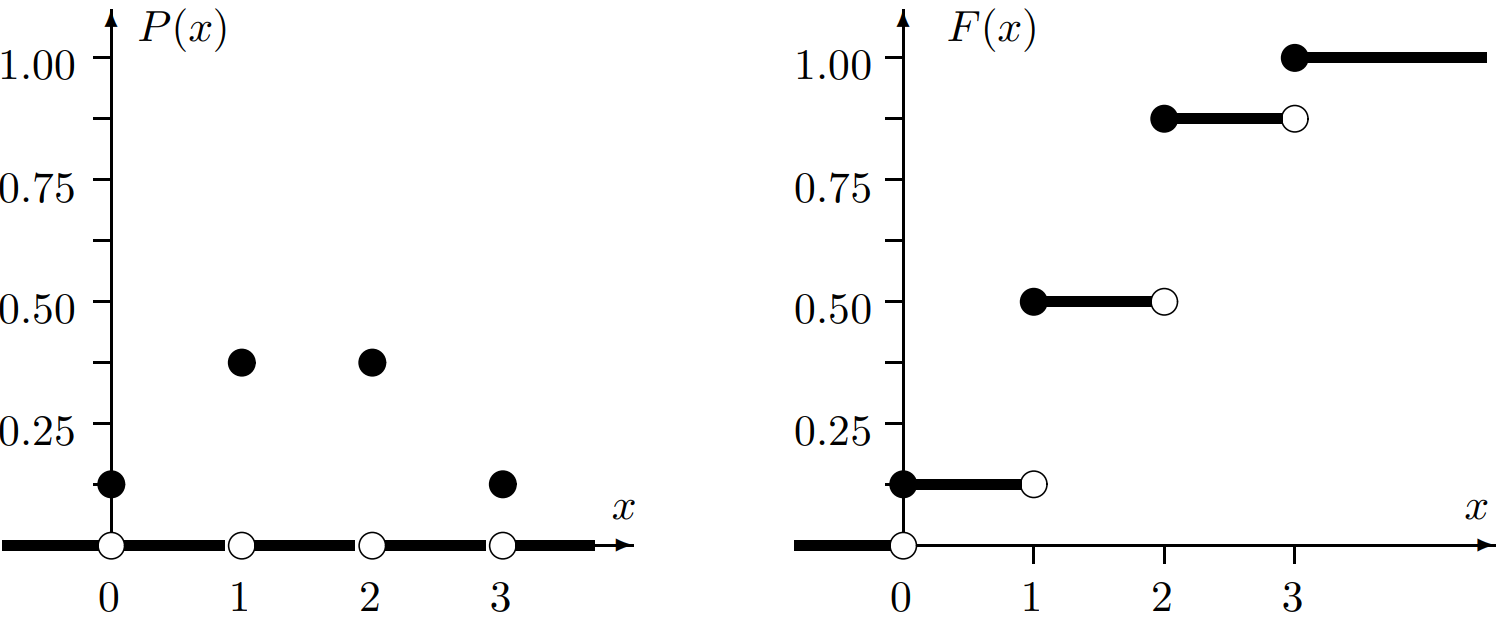
\includegraphics[width=.8\textwidth]{img/fig3.1.png}
    \caption{\textit{The probability mass function $P(x)$ and the cumulative distribution function $F(x)$ for example 1. White circles denote excluded points.}}
\end{figure}

On the obtained histogram, the two middle columns for $X = 1$ and $X = 2$ are about 3 times higher than the columns on each side, for $X = 0$ and $X = 3$. That is, in a run of 10,000 simulations, values 1 and 2 are attained three times more often than 0 and 3. This agrees with the pmf $P(0) = P(3) = 1/8$, $P(1) = P(2) = 3/8$.

\subsection{Types of Random Variables}

So far, we are dealing with \textit{discrete random variables}. These are variables whose range is \textit{finite or countable}. In particular, it means that their values can be listed, or arranged in a sequence. Examples include the number of jobs submitted to a printer, the number of errors, the number of error-free modules, the number of failed components, and so on.

On the contrary, \textit{continuous random variables} assume a whole interval of values. This could be a bounded interval $(a,\ b)$, or an unbounded interval such as $(a,\ +\infty)$, $(-\infty,\ b)$, or $(-\infty,\ +\infty)$. Sometimes, it may be a union of several such intervals. Intervals are uncountable, therefore, all values of a random variable cannot be listed in this case. Examples of continuous variables include various times (software installation time etc., also physical variables like weight, height etc.

\begin{example}{}
For comparison, observe that a long jump is formally a continuous random
variable because an athlete can jump any distance within some range. Results of a high jump, however, are discrete because the bar can only be placed on a finite number of heights. 
\end{example}
Notice that rounding a continuous random variable, say, to the nearest integer makes it discrete.


\section{Distribution of a Random Vector}

Often we deal with several random variables simultaneously. We may look at the size of a RAM and the speed of a CPU, the price of a computer and its capacity, temperature and humidity, technical and artistic performance, etc.

\subsection{Joint Distribution and Marginal Distributions}

\begin{definition}{}
If $X$ and $Y$ are random variables, then the pair $(X,\ Y)$ is a \textbf{random vector}. Its distribution is called the \textbf{joint distribution} of $X$ and $Y$. Individual distributions of $X$ and $Y$ are then called the \textbf{marginal distributions}.
\end{definition}
Generally, we talk about two random variables in this section, all the concepts extend to a vector $(X_1,\ X_2,\ ...,\ X_n)$ of $n$ components and its joint distribution.

Similarly to a single variable, the \textit{joint distribution} of a vector is a collection of probabilities for a vector $(X,\ Y)$ to take a value $(x,\ y)$. Recall that two vectors are equal,
\begin{equation*}
    (X,\ Y) = (x,\ y)
\end{equation*}
if $X = x$ \textbf{\underline{and}} $Y = y$. This ``and'' means the intersection, therefore, the \textit{joint probability mass function} of $X$ and $Y$ is
\begin{equation*}
    P(x,\ y) = \prob{(X,\ Y) = (x,\ y)} = \prob{X = x \cap Y = y}
\end{equation*}
Again, $\{(X,\ Y ) = (x,\ y)\}$ are \textit{exhaustive} and \textit{mutually exclusive} events for different pairs $(x,\ y)$, therefore,
\begin{equation*}
    \sum_x \sum_y P(x,\ y) = 1
\end{equation*}
The joint distribution of $(X,\ Y)$ carries the complete information about the behavior of this random vector. In particular, the marginal probability mass functions of $X$ and $Y$ can be obtained from the joint pmf by the \textit{Addition Rule}.

\begin{formula}{Addition Rule - Eq. 2}
\begin{align*}
    P_X(x) = \prob{X = x} = \sum_y P_{(X,\ Y)} (x,\ y)\\
    P_Y(x) = \prob{Y = y} = \sum_x P_{(X,\ Y)} (x,\ y)\\
\end{align*}
\end{formula}
That is, to get the marginal pmf of one variable, we add the joint probabilities over all values of the other variable.

Events $\{Y = y\}$ for different values of $y$ partition the sample space $\Omega$. Hence, their intersections with $\{X = x\}$ partition the event $\{X = x\}$ into mutually exclusive parts. By the rule for the union of mutually exclusive events, their probabilities should be added. These probabilities are precisely $P_{(X,\ Y)}(x,\ y)$.

In general, the joint distribution cannot be computed from marginal distributions because they carry no information about interrelations between random variables. For example, marginal distributions cannot tell whether variables $X$ and $Y$ are independent or dependent.

\subsection{Independence of Random Variables}

\begin{definition}{}
Random variables $X$ and $Y$ are \textbf{independent} if
\begin{equation*}
    P_{X,\ Y}(x,\ y) = P_X(x) P_Y(y)
\end{equation*}
for all values of $x$ and $y$. This means, events $\{X = x\}$ and $\{Y = y\}$ are independent for all $x$ and $y$; in other words, variables $X$ and $Y$ take their values independently of each other.
\end{definition}
In problems, to show independence of $X$ and $Y$, we have to check whether the joint pmf factors into the product of marginal pmfs for all pairs $x$ and $y$. To prove dependence, we only need to present one counterexample, a pair $(x,\ y)$ with $P(x,\ y) \neq P_X(x) P_Y(y)$.

\begin{example}{2}
A program consists of two modules. The number of errors, $X$, in the first module and the number of errors, $Y$, in the second module have the joint distribution, $P(0,\ 0) = P(0,\ 1) = P(1,\ 0) = 0.2$, $P(1,\ 1) = P(1,\ 2) = P(1,\ 3) = 0.1$, $P(0,\ 2) = P(0,\ 3) = 0.05$. 

Find (a) the marginal distributions of $X$ and $Y$, (b) the probability of no errors in the first module, and (c) the distribution of the total number of errors in the program. Also, (d) find out if errors in the two modules occur independently.

\textbf{Solution:} It is convenient to organize the joint pmf of $X$ and $Y$ in a table. Adding rowwise and columnwise, we get the marginal pmfs (a)
\begin{center}
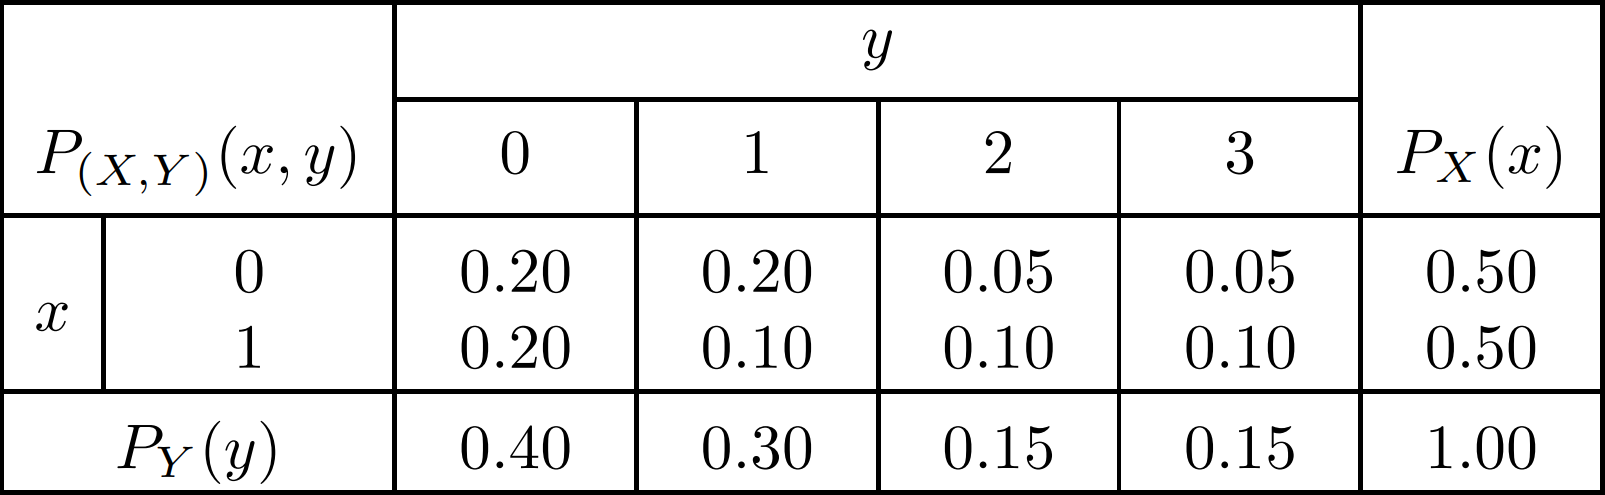
\includegraphics[width=.5\textwidth]{img/table-ex3.6.png}
\end{center}
(b) $P_X (0) = 0.50$.

(c) Let $Z = X + Y$ be the total number of errors. To find the distribution of $Z$, we first identify its possible values, then find the probability of each value. We see that $Z$ can be as small as 0 and as large as 4. Then,
\begin{align*}
    P_Z(0) &= \prob{X + Y = 0} = \prob{X = 0 \cap Y = 0} = P(0,\ 0) = 0.20\\
    P_Z(1) &= \prob{X = 0 \cap Y = 1} + \prob{X = 1 \cap Y = 0} = P(0,\ 1) + P(1,\ 0) = 0.20 + 0.20 = 0.40\\
    P_Z(2) &= P(0,\ 2) + P(1,\ 1) = 0.05 + 0.10 = 0.15\\
    P_Z(3) &= P(0,\ 3) + P(1,\ 2) = 0.05 + 0.10 = 0.15\\
    P_Z(4) &= P(1,\ 3) = 0.10.
\end{align*}
It is a good check to verify that $\sum_z P_Z(z) = 1$

(d) To decide on the independence of $X$ and $Y$, check if their joint pmf factors into a product of marginal pmfs. We can check every pair but it can be seen $P_{(X,\ Y)}(0,\ 1) = 0.2$ whereas $P_X(0)P_Y(1) = (0.5)(0.3) = 0.15$. There is no need to check further. We found a pair of $x$ and $y$ that violates the formula for independent random variables. Therefore, the numbers of errors in two modules are dependent. 
\end{example}


\section{Expectation and variance}

The distribution of a random variable or a random vector, the full collection of related probabilities, contains the entire information about its behavior. This detailed information can be summarized in a few vital characteristics describing the average value, the most likely value of a random variable, its spread, variability, etc. The most commonly used are the \textit{expectation}, \textit{variance}, \textit{standard deviation}, \textit{covariance}, and \textit{correlation}. Also rather popular and useful are the \textit{mode}, \textit{moments}, \textit{quantiles}, and \textit{interquartile range}.

\subsection{Expectation}

\begin{definition}{}
\textbf{Expectation} or \textbf{expected value} of a random variable $X$ is its \textit{mean, the average value}.
\end{definition}

We know that $X$ can take different values with different probabilities. For this reason, its average value is \textit{not} just the average of all its values. Rather, it is a \textit{weighted average}.

\begin{example}{}
Consider a variable that takes values 0 and 1 with probabilities $P(0) =
P(1) = 0.5$. That is,
\begin{equation*}
    X = \begin{cases}
        0 &\text{with the probability 1/2}\\
        1 &\text{with the probability 1/2}
    \end{cases}
\end{equation*}
Observing this variable many times, we shall see $X = 0$ about 50\% of times and $X = 1$ about 50\% of times. The average value of $X$ will then be close to 0.5, so it is reasonable to have $\mathbf{E}(X) = 0.5$.
\end{example}
\noindent Now let’s see how unequal probabilities of $X = 0$ and $X = 1$ affect the expectation $\mathbf{E}(X)$.
\begin{example}{}
Suppose that $P(0) = 0.75$ and $P(1) = 0.25$. Then, in a long run, $X$ is equal
1 only 1/4 of times, otherwise it equals 0. Suppose we earn \$1 every time we see $X = 1$. On the average, we earn \$1 every four times, or \$0.25 per each observation. Therefore, in this case $\mathbf{E}(X) = 0.25$. 
\end{example}

\setcounter{equation}{2}

The general formula for the expectation.
\begin{formula}{Expectation, discrete case}
\begin{equation}
    \mu = \mathbf{E}(X) = \sum_x xP(x)
\end{equation}
\end{formula}
This formula returns the center of gravity for a system with masses $P(x)$ allocated at points $x$. Expected value is often denoted by a Greek letter $\mu$.

In a certain sense, expectation is the best forecast of $X$. The variable itself is random. It takes different values with different probabilities $P(x)$. At the same time, it has just one expectation $\mathbf{E}(X)$ which is non-random.

\subsection{Expectation of a Function}

Often we are interested in another variable, $Y$, that is a function of $X$. For example, downloading time depends on the connection speed, profit of a computer store depends on the number of computers sold, and bonus of its manager depends on this profit. Expectation of $Y = g(X)$ is computed by a similar formula,
\begin{equation}
    \mathbf{E}\{g(x)\} = \sum_x g(x)P(x)
\end{equation}

\textbf{Remark:} Indeed, if $g$ is a one-to-one function, then $Y$ takes each value $y = g(x)$ with probability $P(x)$, and the formula for $E(Y)$ can be applied directly. If $g$ is not one-to-one, then some values of $g(x)$ will be repeated in (eq. 4). However, they are still multiplied by the corresponding probabilities. When we add in (eq. 4), these probabilities are also added, thus each value of $g(x)$ is still multiplied by the probability $P_Y(g(x))$.

\subsection{Properties}

The following linear properties of expectations follow directly from (eq. 3) and (eq. 4). For any random variables $X$ and $Y$ and any non-random numbers $a$, $b$, and $c$, we have
\begin{formula}{Properties of Expectation - Eq. 5}
\begin{align*}
    \mathbf{E}(aX + bY + c) &= a\mathbf{E}(X) + b\mathbf{E}(Y) + c
\end{align*}
In particular,
\begin{align*}
    \mathbf{E}(X + Y) &= \mathbf{E}(X) + \mathbf{E}(Y)\\
    \mathbf{E}(aX) &= a\mathbf{E}(X)\\
    \mathbf{E}(c) &= c
\end{align*}
For \textbf{independent} $X$ and $Y$,
\begin{align*}
    \mathbf{E}(XY) &= \mathbf{E}(X)\mathbf{E}(Y)
\end{align*}
\end{formula}

\textbf{Remark:} The last property in (Eq. 5) holds for some dependent variables too, hence it cannot be used to verify independence of $X$ and $Y$.

\begin{example}{}
In example 2,
\begin{align*}
    \mathbf{E}(X) &= (0)(0.5) + (1)(0.5) = 0.5\\
    \mathbf{E}(Y) &= (0)(0.4) + (1)(0.3) + (2)(0.15) + (3)(0.15) = 1.05
\end{align*}
therefore, the expected total number of errors is
\begin{equation*}
    \mathbf{E}(X + Y ) = 0.5 + 1.05 = 1.65
\end{equation*}
\end{example}
\textbf{Remark:} Clearly, the program will never have 1.65 errors, because the number of errors is always integer. Then, should we round 1.65 to 2 errors? Absolutely not, it would be a mistake. Although both $X$ and $Y$ are integers, their expectations, or average values, do not have to be integers at all.

\subsection{Variance and Standard Deviation}

Expectation shows where the average value of a random variable is located, or where the variable is expected to be, plus or minus some error. How large could this ``error'' be, and how much can a variable vary around its expectation? Let us introduce some measures of variability.

\begin{example}{}
Here is a rather artificial but illustrative scenario. Consider two users. One receives either 48 or 52 e-mail messages per day, with a 50-50\% chance of each. The other receives either 0 or 100 e-mails, also with a 50-50\% chance. What is a common feature of these two distributions, and how are they different?

We see that both users receive the same average number of e-mails:
\begin{equation*}
    \mathbf{E}(X) = \mathbf{E}(Y) = 50
\end{equation*}

However, in the first case, the actual number of e-mails is always close to 50, whereas it always differs from it by 50 in the second case. The first random variable, $X$, is more stable; it has \textit{low variability}. The second variable, $Y$, has \textit{high variability}.
\end{example}

This example shows that variability of a random variable is measured by its distance from the mean $\mu = E(X)$. In its turn, this distance is random too, and therefore, cannot serve as a characteristic of a distribution. It remains to square it and take the expectation of the result.

\begin{definition}{}
\textbf{Variance} of a random variable is defined as the expected squared deviation from the mean. For discrete random variables, variance is
\begin{equation*}
    \sigma^2 = \text{Var}(X) = \mathbf{E}(X - \mathbf{E}X)^2 = \sum_{x} (x - \mu)^2 P(x) 
\end{equation*}
\end{definition}
\textbf{Remark:} Notice that if the distance to the mean is not squared, then the result is always $\mu - \mu = 0$ bearing no information about the distribution of $X$.

According to this definition, variance is always non-negative. Further, it equals 0 only if $x = \mu$ for all values of $x$, i.e., when $X$ is constantly equal to $\mu$. Certainly, a constant (non-random) variable has zero variability. 

\noindent Variance can also be computed as
\begin{equation*}
    \text{Var}(X) = \mathbf{E}(X^2) - \mu^2
\end{equation*}
\begin{definition}{}
\textbf{Standard deviation} is a square root of variance,
\begin{equation*}
    \sigma = \text{Std}(X) = \sqrt{\text{Var}(X)}
\end{equation*}
\end{definition}
\noindent Continuing the Greek-letter tradition, variance is often denoted by $\sigma^2$. Then, standard deviation is $\sigma$.

If $X$ is measured in some units, then its mean $\mu$ has the same measurement unit as $X$. Variance $\sigma^2$ is measured in squared units, and therefore, it cannot be compared with $X$ or $\mu$. No matter how funny it sounds, it is rather normal to measure variance of profit in squared dollars, variance of class enrollment in squared students, and variance of available disk space in squared gigabytes. When a squared root is taken, the resulting standard deviation $\sigma$ is again measured in the same units as $X$. This is the main reason of introducing yet another measure of variability, $\sigma$.

\subsection{Covariance and Correlation}

Expectation, variance, and standard deviation characterize the distribution of a single random variable. Now we introduce measures of \textit{association} of two random variables.

\begin{definition}{}
\textbf{Covariance} $\sigma_{XY}$ = Cov$(X,\ Y)$ is defined as
\begin{align*}
    \text{Cov}(X,\ Y) &= \mathbf{E}\{(X - \mathbf{E}X) (Y - \mathbf{E}Y)\}\\
    &= \mathbf{E}(XY) - \mathbf{E}(X)\mathbf{E}(Y)
\end{align*}
It summarizes interrelation of two random variables.
\end{definition}

Covariance is the expected product of deviations of $X$ and $Y$ from their respective expectations. If Cov$(X,\ Y) > 0$, then positive deviations $(X - \mathbf{E}X)$ are more likely to be multiplied by positive $(Y - \mathbf{E}Y)$, and negative $(X - \mathbf{E}X)$ are more likely to be multiplied by negative $(Y - \mathbf{E}Y)$. In short, large $X$ imply large $Y$, and small $X$ imply small $Y$. These variables are \textit{\textbf{positively correlated}}.

Conversely, Cov$(X,\ Y) < 0$ means that large $X$ generally correspond to small $Y$ and small $X$ correspond to large $Y$. These variables are \textit{\textbf{negatively correlated}}.

If Cov$(X,\ Y) = 0$, we say that $X$ and $Y$ are \textit{\textbf{uncorrelated}}.

These can be seen in the figure 2, (a), (b) and (c), respectively.

\begin{figure}[t]
    \centering
    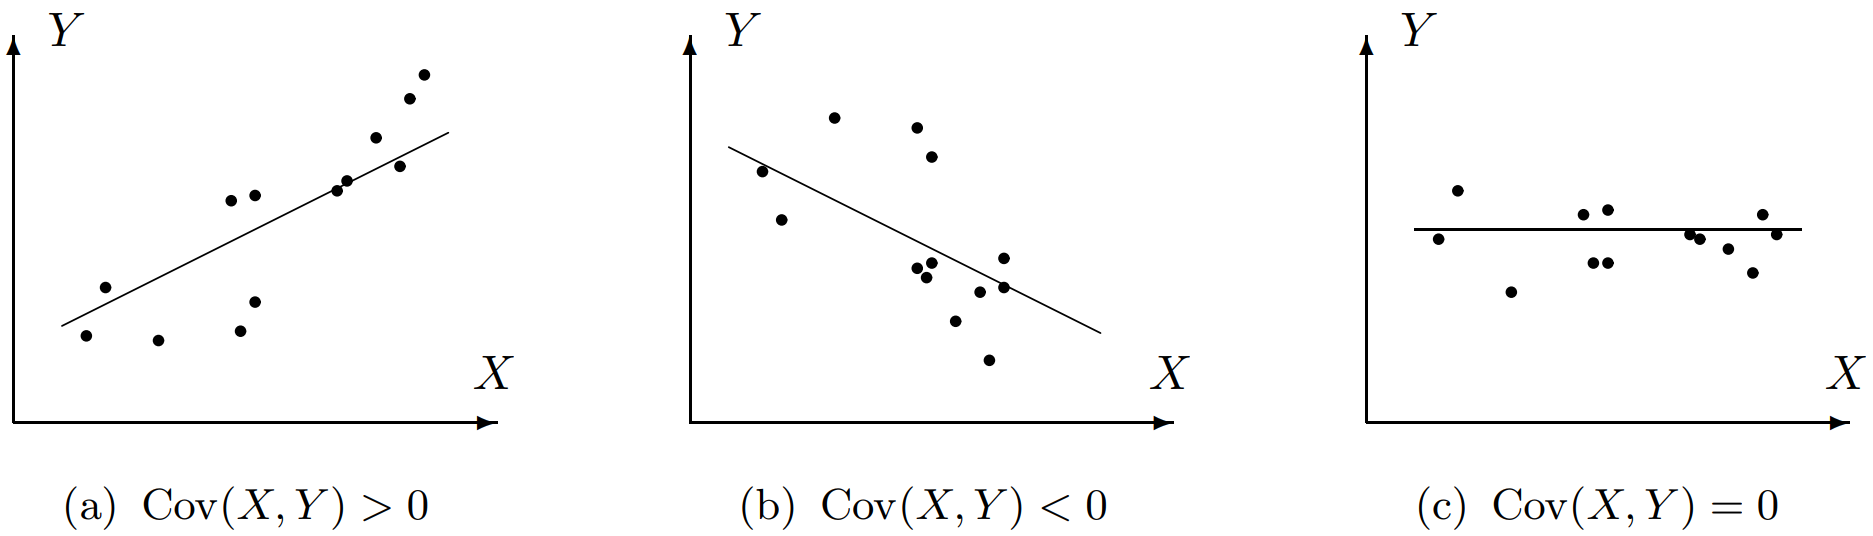
\includegraphics[width=.6\textwidth]{img/fig3.4.png}
    \caption{\textit{Positive, negative, and zero covariance.}}
\end{figure}

\begin{definition}{}
\textbf{Correlation coefficient} between variables $X$ and $Y$ is defined as
\begin{equation*}
    \rho = \frac{\text{Cov}(X,\ Y)}{(\text{Std$X$})(\text{Std$Y$})}
\end{equation*}
\end{definition}

Correlation coefficient is a rescaled, normalized covariance. Notice that covariance Cov$(X,\ Y)$ has a measurement unit. It is measured in units of $X$ multiplied by units of $Y$. As a result, it is not clear from its value whether $X$ and $Y$ are strongly or weakly correlated. Really, one has to compare Cov$(X,\ Y)$ with the magnitude of $X$ and $Y$. Correlation coefficient performs such a comparison, and as a result, it is dimensionless.

How do we interpret the value of $\rho$? What possible values can it take? As a special case of famous Cauchy-Schwarz inequality,
\begin{equation*}
    -1 \leq \rho \leq 1
\end{equation*}
where $|\rho| = 1$ is possible only when all values of $X$ and $Y$ lie on a straight line, as in Figure 3. Further, values of $\rho$ near 1 indicate strong positive correlation, values near (-1) show strong negative correlation, and values near 0 show weak correlation or no correlation.

\begin{figure}[h!]
    \centering
    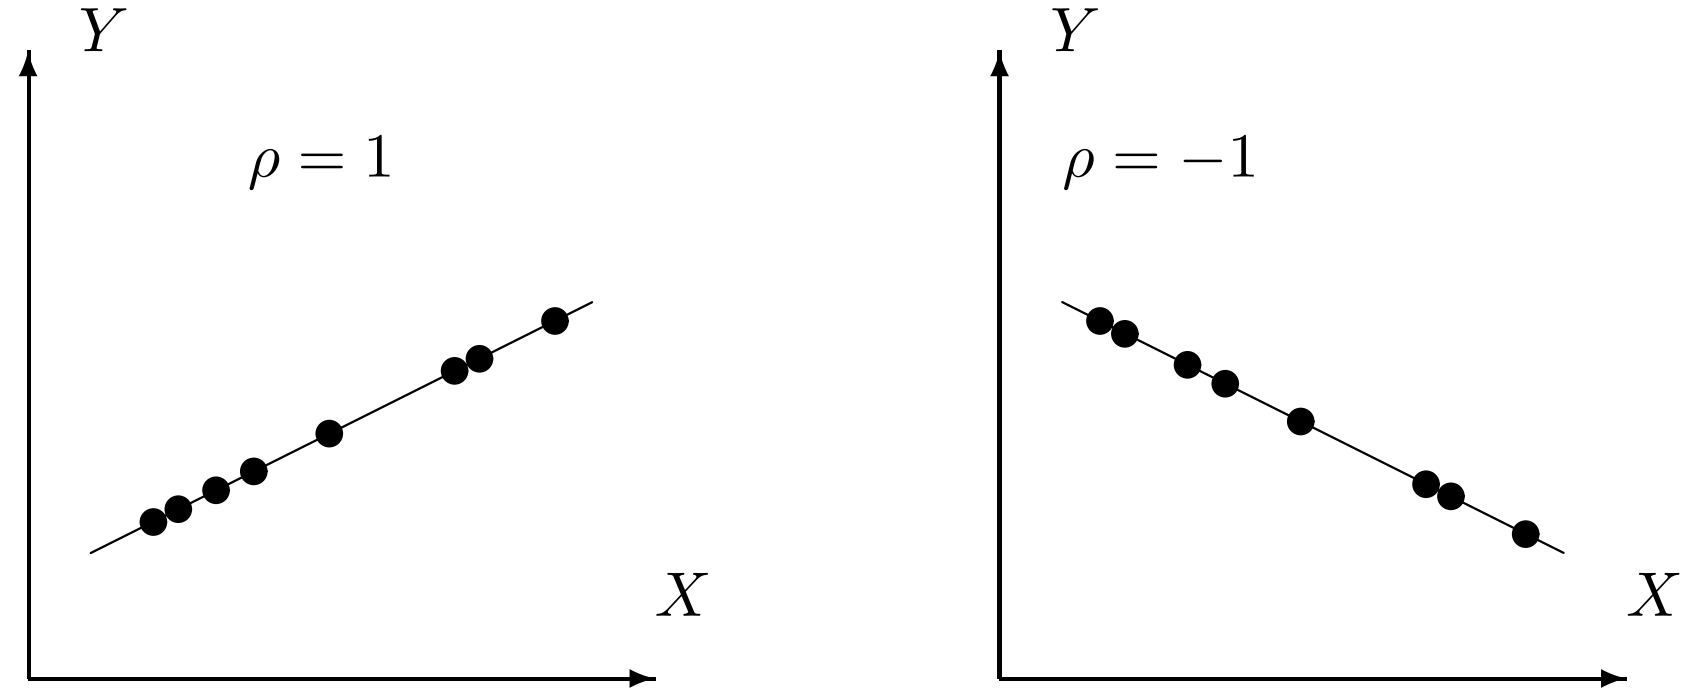
\includegraphics[width=.4\textwidth]{img/fig3.5.png}
    \caption{\textit{Perfect correlation: $\rho = \pm 1$.}}
\end{figure}

\subsection{Properties}

The following properties of variances, covariances, and correlation coefficients hold for any random variables $X$, $Y$, $Z$, and $W$ and any non-random numbers $a$, $b$, $c$ and $d$.
\begin{formula}{Properties of Variances and Covariances - Eq. 7}
\begin{align*}
    \text{Var}(aX + bY + c) &= a^2\text{Var}(X) + b^2\text{Var}(Y) + 2ab\text{Cov}(X,\ Y)\\ \text{Cov}(aX + bY,\ cZ + dW) &= ac\text{Cov}(X,\ Z) + ad\text{Cov}(X,\ W) + bc\text{Cov}(Y,\ Z) + bd\text{Cov}(Y,\ W)\\
    \text{Cov}(X,\ Y) &= \text{Cov}(Y,\ X)\\
    \rho(X,\ Y) &= \rho(Y,\ X)
\end{align*}
In particular,
\begin{align*}
    \text{Var}(aX + b) &= a^2\text{Var}(X)\\
    \text{Cov}(aX + b,\ cY + d) &= ac\text{Cov}(X,\ Y)\\
    \rho(aX + b,\ cY + d) &= \rho(X,\ Y)
\end{align*}
For independent $X$ and $Y$,
\begin{align*}
    \text{Cov}(X,\ Y) &= 0\\
    \text{Var}(X + Y) &= \text{Var}(X) + \text{Var}(Y)
\end{align*}
\end{formula}

\begin{proof}
To prove the first two formulas, we only need to multiply parentheses in the definitions of \textit{variance} and \textit{covariance} and apply (eq. 5):
\begin{align*}
    \text{Var}(aX + bY + c) &= \mathbf{E}\{aX + bY + c - \mathbf{E}(aX + bY + c)\}^2\\
    &= \mathbf{E}\{(aX - a \mathbf{E}X) + (bY - b\mathbf{E}Y ) + (c - c)\}^2\\
    &= \mathbf{E}\{a(X - \mathbf{E}X)\}^2 + \mathbf{E}\{b(Y - \mathbf{E}Y)\}^2 + \mathbf{E}\{a(X - \mathbf{E}X)b(Y - \mathbf{E}Y)\} + \mathbf{E}\{b(Y - \mathbf{E}Y)a(X - \mathbf{E}X)\}\\
    &= a^2 \text{Var}(X) + b^2 \text{Var}(Y) + 2ab\text{Cov}(X,\ Y )
\end{align*}

For independent $X$ and $Y$ , we have $\mathbf{E}(XY) = \mathbf{E}(X) \mathbf{E}(Y)$ from (eq. 5). Then, according to the definition of covariance, Cov$(X,\ Y) = 0$.
\end{proof}

We see that \textit{independent variables are always uncorrelated}. The reverse is not always true. There exist some variables that are uncorrelated but not independent.

Notice that adding a constant does not affect the variables’ variance or covariance. It shifts the whole distribution of $X$ without changing its variability or degree of dependence of another variable. The correlation coefficient does not change even when multiplied by a constant because it is recomputed to the unit scale, due to Std($X$) and Std($Y$) in the denominator in definition of ``Correlation coefficient''.

\begin{mybox}[breakable]{green}{\textbf{Example}}
    Continuing Example 2, we compute
    \begin{center}
    \begin{tabular}{|c|c|c|c|c|}
    $x$ & $P_X(x)$ & $xP_X(x)$            & $x-\mathbf{E}X$ & $(x-\mathbf{E}X)^2P_X(x)$  \\ 
    \hline
    0   & 0.5      & 0                    & -0.5            & 0.125                      \\
    2   & 0.5      & 0.5                  & 0.5             & 0.125                      \\ 
    \hline
    \multicolumn{3}{|c|}{$\mu_X = 0.5$}   & \multicolumn{2}{c|}{$\sigma_X^2 = 0.25$}    
    \end{tabular}
    \end{center}
    and (using the second method of computing variances)
    \begin{center}
    \begin{tabular}{|c|c|c|c|c|}
    $y$ & $P_Y(y)$ & $yP_Y(y)$            & $y^2$ & $y^2P_Y(y)$                            \\ 
    \hline
    0   & 0.4      & 0                    & 0     & 0                                      \\
    1   & 0.3      & 0.3                  & 1     & 0.3                                    \\
    2   & 0.15     & 0.3                  & 4     & 0.6                                    \\
    3   & 0.15     & 0.45                 & 9     & 1.35                                   \\ 
    \hline
    \multicolumn{3}{|c|}{$\mu_Y = 1.05$}   & \multicolumn{2}{c|}{$\mathbf{E}(Y^2) = 2.25$} 
    \end{tabular}
    \end{center}
    
    \newpage
    \textbf{\textit{Result:}} Var$(X) = 0.25$, Var$(Y) = 2.25 - 1.05^2 = 1.1475$, Std$(X) = \sqrt{0.25} = 0.5$, and Std$(Y) = \sqrt{1.1475} = 1.0712$. Also,
    \begin{equation*}
        \mathbf{E}(XY) = \sum_x \sum_y xy P(x,\ y) = (1)(1)(0.1) + (1)(2)(0.1) + (1)(3)(0.1) = 0.6
    \end{equation*}
    (the other five terms in this sum are 0). Therefore,
    \begin{equation*}
        \text{Cov}(X,\ Y) = \mathbf{E}(XY) - \mathbf{E}(X)\mathbf{E}(Y) = 0.6 - (0.5)(1.05) = 0.075
    \end{equation*}
    and
    \begin{equation*}
        \rho = \frac{\text{Cov}(X,\ Y)}{(\text{Std}X)(\text{Std}Y)} = \frac{0.075}{(0.5)(1.0712)} = 0.1400
    \end{equation*}
    
    Thus, the numbers of errors in two modules are positively and not very strongly correlated.
\end{mybox}

\textbf{NOTATION}
\begin{align*}
    \mu \text{ or } \mathbf{E}(X) &= \text{expectation}\\
    \sigma_X^2 \text{ or Var}(X) &= \text{variance}\\
    \sigma_X \text{ or Std}(X) &= \text{standard deviation}\\
    \sigma_{XY} \text{ or Cov}(X,\ Y) &= \text{covariance}\\
    \rho_{XY} &= \text{correlation coefficient}
\end{align*}


\section{Families of Discrete Distributions}

\subsection{Bernoulli Distribution}

The simplest random variable (excluding non-random ones!) takes just two possible values. Call them 0 and 1.

\begin{definition}{}
A random variable with two possible values, 0 and 1, is called a \textbf{Bernoulli variable}, its distribution is \textbf{Bernoulli distribution}, and any experiment with a \textit{binary outcome} is called a \textbf{Bernoulli trial}.
\end{definition}

Good or defective components, parts that pass or fail tests, transmitted or lost signals, working or malfunctioning hardware, benign or malicious attachments, sites that contain or do not contain a keyword, girls and boys, heads and tails, and so on, are examples of Bernoulli trials. All these experiments fit the same Bernoulli model, where we shall use generic names for the two outcomes: ``\textit{successes}'' and ``\textit{failures}''. These are nothing but commonly used generic names; in fact, successes do not have to be good, and failures do not have to be bad.

If $P(1) = p$ is the probability of a \textit{success}, then $P(0) = q = 1 - p$ is the probability of a \textit{failure}. We can then compute the expectation and variance as
\begin{align*}
    \mathbf{E}(X) &= \sum_{x} P(x) = (0)(1-p) + (1)(p) = p\\
    \text{Var}(X) &= \sum_{x} (x-p)^2P(x) = (0-p)^2(1-p) + (1-p)^2p\\
    &= p(1-p)(p+1-p) = p(1-p)
\end{align*}

\begin{formula}{Bernoulli Distribution}
\begin{align*}
    p &= \text{probability of success}\\
    P(x) &= \begin{cases}
                q = 1-p &\text{if $x = 0$}\\
                p &\text{if $x=1$}
            \end{cases}\\
    \mathbf{E}(X) &= p\\
    \text{Var}(X) &= pq\ \ [=p (1-p)]
\end{align*}
\end{formula}

In fact, we see that there is a whole family of Bernoulli distributions, indexed by a parameter $p$. Every $p$ between 0 and 1 defines another Bernoulli distribution. The distribution with $p = 0.5$ carries the highest level of uncertainty because Var$(X) = pq$ is maximized by $p = q = 0.5$. Distributions with lower or higher $p$ have lower variances. Extreme parameters $p = 0$ and $p = 1$ define non-random variables 0 and 1, respectively; their variance is 0.

\subsection{Binomial Distribution}

Now consider a sequence of independent Bernoulli trials and count the number of successes in it. This may be the number of defective computers in a shipment, the number of updated files in a folder, the number of girls in a family, the number of e-mails with attachments, etc.

\begin{definition}{}
A variable described as the number of successes in a sequence of independent Bernoulli trials has \textbf{Binomial distribution}. Its parameters are $n$, the number of trials, and $p$, the probability of success.
\end{definition}

\textbf{Remark:} ``\texttt{Binomial}'' can be translated as ``two numbers'', \textit{bi} meaning ``two'' and \textit{nom} meaning ``a number'', thus reflecting the concept of binary outcomes.

Binomial probability mass function is
\setcounter{equation}{8}
\begin{equation}
    P(x) = \prob{X = x} = \binom{n}{x}p^xq^{n-x},\ \ \ \ x = 0, 1, ..., n
\end{equation}
which is the probability of exactly $x$ \textit{successes} in $n$ trials. In this formula, $p^x$ is the probability of $x$ \textit{successes}, probabilities being multiplied due to independence of trials. Also, $q^{n-x}$ is the probability of the remaining $(n - x)$ trials being failures. Finally, $\dbinom{n}{x} = \dfrac{n!}{x! (n-x)!}$ is the number of elements of the sample space $\Omega$ that form the event $\{X = x\}$. This is the number of possible orderings of $x$ successes and $(n - x)$ failures among $n$ trials, and it is computed as $C(n, x)$.

Due to a somewhat complicated form of (eq. 9), practitioners use a table of \textit{Binomial distribution}, Table A2 (in book page 412). Its entries are values of the Binomial cdf $F(x)$. If we need a pmf instead of a cdf, we can always compute it from the table as
\begin{equation*}
    P(x) = F(x) - F(x - 1)
\end{equation*}

Let’s turn to the Binomial expectation and variance. Computing the expected value directly by (eq. 3) results in a complicated formula,
\begin{equation*}
    \mathbf{E}(X) = \sum_{x=0}^{n} x \binom{n}{x} p^x q^{n-x} = ... ?
\end{equation*}
A shortcut can be obtained from the following important property.

Each Bernoulli trial is associated with a Bernoulli variable that equals 1 if the trial results in a success and 0 in case of a failure. Then, a sum of these variables is the overall number
of successes. Thus, any \textit{Binomial variable} $X$ can be represented as a sum of independent \textit{Bernoulli variables},
\begin{equation*}
    X = X_1 + ... + X_n
\end{equation*}
We can use this to compute (referring to (eq. 5) and (eq. 7))
\begin{align*}
    \mathbf{E}(X) &= \mathbf{E}(X_1 + ... + X_n) = \mathbf{E}(X_1) + ... + \mathbf{E}(X_n) = p + ... + p = np\\
    \text{Var}(X) &= \text{Var}(X_1 + ... + X_n) = \text{Var}(X_1) + ... + \text{Var}(X_n) = npq
\end{align*}

\begin{formula}{Binomial Distribution}
\begin{align*}
    n &= \text{number of trials}\\
    p &= \text{probability of success}\\
    P(x) &= \binom{n}{x} p^x q^{n-x}\\
    \mathbf{E}(X) &= np\\
    \text{Var}(X) &= npq
\end{align*}
\end{formula}

\begin{example_break}{}
An exciting computer game is released. Sixty percent of players complete all the levels. Thirty percent of them will then buy an advanced version of the game. Among 15 users, what is the expected number of people who will buy the advanced version? What is the probability that at least two people will buy it?

\newpage
\textbf{Solution:}
Let $X$ be the number of people (successes), among the mentioned 15 users (trials), who will buy the advanced version of the game. It has Binomial distribution with $n = 15$ trials and the probability of success
\begin{align*}
    p &= \prob{\text{buy advanced}}\\
    &= \prob{\text{buy advanced $|$ complete all levels}} \prob{\text{complete all levels}}\\
    &= (0.30)(0.60) = 0.18.
\end{align*}

Then we have
\begin{equation*}
    \mathbf{E}(X) = np = (15)(0.18) = 2.7
\end{equation*}
and
\begin{equation*}
    \prob{X \geq 2} = 1 - P(0) - P(1) = 1 - (1 - p)^n - np(1 - p)^{n-1} = 0.7813.
\end{equation*}
The last probability was computed directly by formula (eq. 9).
\end{example_break}

\subsection{Geometric Distribution}

Consider a sequence of independent Bernoulli trials. Each trial results in a ``success'' or a ``failure''.
\begin{definition}{}
The number of Bernoulli trials needed to get the first success has \textbf{Geometric distribution}.
\end{definition}

\noindent \textbf{Mini Examples:}
\begin{itemize}
    \item A search engine goes through a list of sites looking for a given key phrase. Suppose the search terminates as soon as the key phrase is found. The number of sites visited is Geometric.
    \item A hiring manager interviews candidates, one by one, to fill a vacancy. The number of candidates interviewed until one candidate receives an offer has Geometric distribution.
\end{itemize}

Geometric random variables can take any integer value from 1 to infinity, because one needs at least 1 trial to have the first success, and the number of trials needed is not limited by any specific number. (For example, there is no guarantee that among the first 10 coin tosses there will be at least one head.) The only parameter is $p$, the probability of a ``success''.

Geometric probability mass function has the form
\begin{equation*}
    P(x) = \prob{\text{the 1st success occurs on the $x$-th trial}} = (1-p)^{x-1}p,\ \ \ \ x = 1, 2, ...
\end{equation*}
which is the probability of $(x - 1)$ failures followed by one success. Comparing with (eq.9), there is no number of combinations in this formula because only one outcome has the first success coming on the $x$-th trial.

This is the first time we see an \textit{unbounded} random variable, that is, with no upper bound. Variable $X$ can take any positive integer value, from 1 to $\infty$. It is insightful to check whether
$\sum_x P(x) = 1$, as it should hold for all pmf. Indeed,
\begin{equation*}
    \sum_x P(x) = \sum_{x=1}^{\infty} (1-p)^{x-1} p = \frac{(1-p)^0}{1 - (1-p)} p = 1
\end{equation*}
where we noticed that the sum on the left is a \textit{geometric series} that gave its name to Geometric distribution.

Finally, Geometric distribution has expectation $\mu = 1/p$ and variance $\sigma^2 = (1 - p)/p^2$.

\textit{Proof of this can be and should be read from book. It is related to geometric series properties.}

\begin{formula}{Geometric Distribution - Eq. 10}
\begin{align*}
    p &= \text{probability of success}\\
    P(x) &= (1-p)^{x-1} p,\ \ x = 1, 2, ...\\
    \mathbf{E}(X) &= \frac{1}{p}\\
    \text{Var}(X) &= \frac{1-p}{p^2}
\end{align*}
\end{formula}

\textit{In book, there is an example of \textit{St. Petersburg Paradox}. This example should be read from book, page 62.}

\subsection{Negative Binomial Distribution}

When we studied Geometric distribution and St. Petersburg paradox in Section 4.3, we played a game until the first win. Now keep playing until we reach $k$ wins. The number of games played is then \textit{Negative Binomial}.

\begin{definition}{}
In a sequence of independent Bernoulli trials, the number of trials needed to obtain $k$ successes has \textbf{Negative Binomial distribution}.
\end{definition}

In some sense, Negative Binomial distribution is opposite to Binomial distribution. Binomial variables count the number of successes in a fixed number of trials whereas Negative Binomial variables count the number of trials needed to see a fixed number of successes. Other than this, there is nothing ``negative'' about this distribution.

Negative Binomial probability mass function is
\begin{align*}
    P(x) &= \prob{\text{ the $x$-th trial results in the $k$-th success }}\\
    &= \prob{(k-1) \text{   successes in the first $(x - 1)$ trials, and the last trial is a success}}\\
    &= \binom{x-1}{k-1} (1 - p)^{x-k} p^k
\end{align*}

This formula accounts for the probability of $k$ successes, the remaining $(x - k)$ failures, and the number of outcomes–sequences with the $k$-th success coming on the $x$-th trial.

Negative Binomial distribution has two parameters, $k$ and $p$. With $k = 1$, it becomes Geometric. Also, each Negative Binomial variable can be represented as a sum of independent Geometric variables,
\setcounter{equation}{10}
\begin{equation}
    X = X_1 + ... + X_k,
\end{equation}
with the same probability of success $p$. Indeed, the number of trials until the $k$-th success consists of a Geometric number of trials $X_1$ until the first success, an additional Geometric
number of trials $X_2$ until the second success, etc.

Because of (eq. 11), we have,
\begin{align*}
    \mathbf{E}(X) &= \mathbf{E}(X_1 + ... + X_k) =\frac{k}{p}\\
    \text{Var}(X) &= \text{Var}(X_1 + ... + X_k) = \frac{k (1 - p)}{p^2}
\end{align*}

\begin{formula}{Negative Binomial Distribution - Eq. 12}
\begin{align*}
    k &= \text{number of success}\\
    p &= \text{probability of success}\\
    P(x) &= (1-p)^{x-k} p^k,\ \ \ \ x = k, k+1, ...\\
    \mathbf{E}(X) &= \frac{k}{p}\\
    \text{Var}(X) &= \frac{k (1-p)}{p^2}
\end{align*}
\end{formula}

\begin{example_break}{Sequential testing}
In a recent production, 5\% of certain electronic components are defective. We need to find 12 non-defective components for our 12 new
computers. Components are tested until 12 non-defective ones are found. What is the probability that more than 15 components will have to be tested?

\textbf{Solution:}
Let $X$ be the number of components tested until 12 non-defective ones are found. It is a number of trials needed to see 12 successes, hence $X$ has \textit{Negative Binomial distribution} with $k = 12$ and $p = 0.05$.

We need $\prob{X > 15} = \sum_{16}^{\infty} P(x)$ or $1 - F(15)$; however, there is no table of Negative Binomial distribution, and applying the formula for $P(x)$ directly is rather cumbersome. What would be a quick solution?

\newpage
Virtually any Negative Binomial problem can be solved by a Binomial distribution. Although $X$ is not Binomial at all, the probability $\prob{X > 15}$ can be related to some Binomial variable. In our example,
\begin{align*}
    \prob{X > 15} &= \prob{\text{ more than 15 trials needed to get 12 successes }}\\
    &= \prob{\text{ 15 trials are not sufficient }}\\
    &= \prob{\text{ there are fewer than 12 successes in 15 trials }}\\
    &= \prob{Y < 12}
\end{align*}
where $Y$ is the number of successes (non-defective components) in 15 trials, which is a Binomial variable with parameters $n = 15$ and $p = 0.95$. 
\begin{equation*}
    \prob{X > 15} = \prob{Y < 12} = \prob{Y \leq 11} = F(11) = 0.0055
\end{equation*}

This technique, expressing a probability about one random variable in terms of another random variable, is rather useful. Soon it will help us relate Gamma and Poisson distributions and simplify computations significantly. 
\end{example_break}

\subsection{Poisson Distribution}

The next distribution is related to a concept of \textit{rare events}, or \textit{Poissonian events}. Essentially it means that two such events are extremely unlikely to occur simultaneously or within a very short period of time. Arrivals of jobs, telephone calls, e-mail messages, traffic accidents, network blackouts, virus attacks, errors in software, floods, and earthquakes are examples of rare events.
\begin{definition}{}
The number of rare events occurring within a fixed period of time has \textbf{Poisson distribution}.
\end{definition}

\begin{formula}{Poisson Distribution}
\begin{align*}
    \lambda &= \text{frequency, average number of events}\\
    P(x) &= e^{-\lambda} \frac{\lambda^x}{x!},\ \ \ x = 1, 2, ...\\
    \mathbf{E}(X) &= \lambda\\
    \text{Var}(X) &= \lambda
\end{align*}
\end{formula}

A Poisson variable can take any nonnegative integer value because there may be no rare events within the chosen period, on one end, and the possible number of events is not limited, on the other end. Poisson distribution has one parameter, $\lambda > 0$, which is the
average number of the considered rare events. Values of its cdf are given in Table A3 on book p. 415.

\begin{example}{New accounts}
Customers of an internet service provider initiate new accounts at the average rate of 10 accounts per day.

(a) What is the probability that more than 8 new accounts will be initiated today?
(b) What is the probability that more than 16 accounts will be initiated within 2 days?

\textbf{Solution:}
(a) New account initiations qualify as rare events because no two customers open accounts simultaneously. Then the number $X$ of today’s new accounts has Poisson distribution with parameter $\lambda = 10$. From Table A3,
\begin{equation*}
    \prob{X > 8} = 1 - F_X (8) = 1 - 0.333 = 0.667
\end{equation*}

(b) The number of accounts, $Y$ , opened within 2 days does not equal $2X$. Rather, $Y$ is another Poisson random variable whose parameter equals 20. Indeed, the parameter is the average number of rare events, which, over the period of two days, doubles the one-day average. Using Table A3 with $\lambda = 20$,
\begin{equation*}
    \prob{Y > 16} = 1 - F_Y (16) = 1 - 0.221 = 0.779
\end{equation*}
\end{example}

\newpage
\subsection{Poisson Approximation of Binomial Distribution}

Poisson distribution can be effectively used to approximate Binomial probabilities when the number of trials $n$ is large, and the probability of success $p$ is small. Such an approximation is adequate, say, for $n \geq 30$ and $p \leq 0.05$, and it becomes more accurate for larger $n$.
\begin{example}{New accounts, continued}
Indeed, the situation in example named ``new accounts'' can be viewed as a sequence of Bernoulli trials. Suppose there are $n = 400,000$ potential internet users in the area, and on any specific day, each of them opens a new account with probability $p = 0.000025$. We see that the number of new accounts is the number of successes, hence a Binomial model with expectation $\mathbf{E}(X) = np = 10$ is possible. However, a distribution with such extreme $n$ and $p$ is unlikely to be found in any table, and computing its pmf by hand is tedious. Instead, one can use Poisson distribution with the same expectation $\lambda = 10$.
\end{example}

\setcounter{equation}{13}
\begin{formula}{Poisson Approximation to Binomial}
\begin{align}
    \texttt{Binomial}(n, p) \approx Poisson(\lambda)& &\text{where $n \geq 30$, $p \leq 0.05$, $np = \lambda$}
\end{align}
\end{formula}
\textbf{Remark:} Mathematically, it means closeness of Binomial and Poisson pmf
\begin{equation*}
    \lim_{\substack{n \to \infty \\ p\to0 \\ np\to\lambda}} \binom{n}{x} p^x (1-p)^{n-x} = e^{- \lambda} \frac{\lambda^x}{x!}
\end{equation*}
and this is what S. D. Poisson has shown.

When p is large $(p \geq 0.95)$, the Poisson approximation is applicable too. The probability of a failure $q = 1 - p$ is small in this case. Then, we can approximate the number of failures, which is also Binomial, by a Poisson distribution.

\begin{example}{}
Ninety-seven percent of electronic messages are transmitted with no error. What is the probability that out of 200 messages, at least 195 will be transmitted correctly?

\textbf{Solution:}
Let $X$ be the number of correctly transmitted messages. It is the number of successes in 200 Bernoulli trials, thus $X$ is Binomial with $n = 200$ and $p = 0.97$. Poisson approximation cannot be applied to $X$ because $p$ is too large. However, the number of failures $Y$ is also Binomial, with parameters $n = 200$ and $q = 0.03$, and it is approximately Poisson with $\lambda = nq = 6$. From Table A3
\begin{equation*}
    \prob{X \geq 195} = \prob{Y \leq 5} = F_Y (5) \approx 0.446.
\end{equation*}
\end{example}

There is a great variety of applications involving a large number of trials with a small probability of success. If the trials are not independent, the number of successes is not Binomial, in general. However, if dependence is weak, the use of Poisson approximation in such problems can still produce remarkably accurate results.


The introduced method can only be applied to very small and very large values of $p$. For moderate $p$ $(0.05 \leq p \leq 0.95)$, the Poisson approximation may not be accurate. These cases are covered by the Central Limit Theorem (later).

\end{document}
